\documentclass[a4paper, 11pt]{article}
\usepackage[margin=3cm]{geometry}
\usepackage[]{fontenc}
\usepackage[utf8]{inputenc}
\usepackage[italian]{babel}
\usepackage{geometry}
\geometry{a4paper, top=2cm, bottom=3cm, left=1.5cm, right=1.5cm, heightrounded, bindingoffset=5mm}
\usepackage{amsmath}
\usepackage{amssymb}
\usepackage{gensymb}
\usepackage{graphicx}
\usepackage{psfrag,amsmath,amsfonts,verbatim}
\usepackage{xcolor}
\usepackage{color,soul}
\usepackage{fancyhdr}
\usepackage{indentfirst}
\usepackage{graphicx}
\usepackage{newlfont}
\usepackage{latexsym}
\usepackage{amsthm}
%\usepackage{subfigure}
\usepackage{subcaption}
\usepackage{psfrag}
\usepackage{footnote}
\usepackage{graphics}
\usepackage{color}
\usepackage{hyperref}
\usepackage{tikz}
\usepackage{float}


\usetikzlibrary{snakes}
\usetikzlibrary{positioning}
\usetikzlibrary{shapes,arrows}

	
	\tikzstyle{block} = [draw, fill=white, rectangle, 
	minimum height=3em, minimum width=6em]
	\tikzstyle{sum} = [draw, fill=white, circle, node distance=1cm]
	\tikzstyle{input} = [coordinate]
	\tikzstyle{output} = [coordinate]
	\tikzstyle{pinstyle} = [pin edge={to-,thin,black}]

\newcommand{\courseacronym}{CAT}
\newcommand{\coursename}{Controlli Automatici - T}
\newcommand{\tipology}{A }
\newcommand{\trace}{1}
\newcommand{\projectname}{Controllo dell'assetto di un drone planare}
\newcommand{\group}{Q}

%opening
\title{ \vspace{-1in}
		\huge \strut \coursename \strut 
		\\
		\Large  \strut Progetto Tipologia \tipology - Traccia \trace 
		\\
		\Large  \strut \projectname\strut
		\\
		\Large  \strut Gruppo \group\strut
		\vspace{-0.4cm}
}
\author{Clarissa Bovo, Fabio Cangiano, Francesca Porzia Fedi, Antonio Zara}
\date{}

\begin{document}

\maketitle
\vspace{-0.5cm}

Il progetto riguarda il controllo dell'assetto di un drone planare, la cui dinamica viene descritta dalle seguenti equazioni differenziali 
%
\begin{subequations}\label{eq:system}
\begin{align}
	\dot{\theta}&=\omega \\
    J\dot{\omega}&=-\beta\omega+\frac{a}{2}\sin{(\theta)}F_v+a F_p
\end{align}
\end{subequations}
%

\begin{figure}[H]
    \centering
    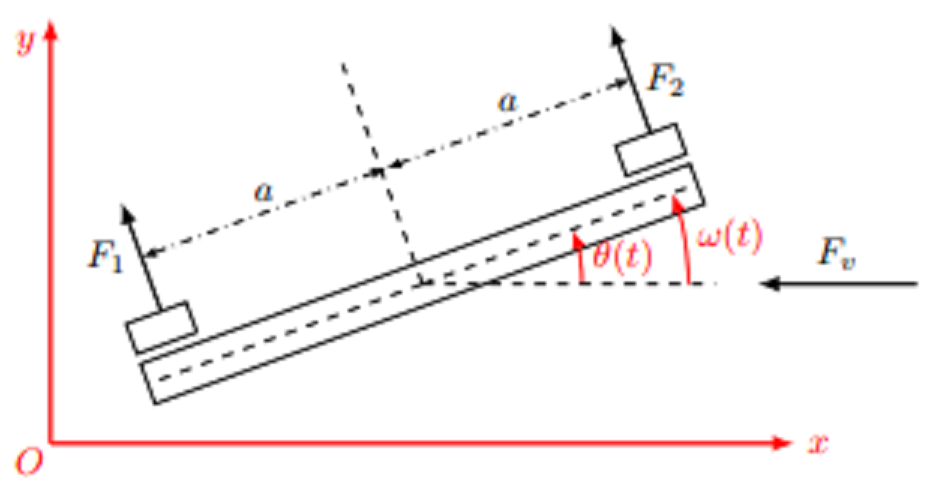
\includegraphics[width=0.4\textwidth]{immagini/figura_drone.png}
    \caption{Rappresentazione nel piano del drone considerato}
    \label{fig:figura_drone}
\end{figure}

Dove:
\begin{itemize}
    \item $\theta$ rappresenta l'angolo di inclinazione rispetto al piano.
    \item $\omega$ rappresenta la velocità di rotazione rispetto all’asse perpendicolare
al piano passante per il baricentro
    \item $J$ rappresenta il momento di inerzia del drone rispetto all’asse di
rotazione che passa per il baricentro
    \item $\beta$ rappresenta il coefficiente d’attrito dinamico dovuto alla presenza
dell’aria
    \item $a$ rappresenta la semi-ampiezza planare del drone
    \item $F_v$ rappresenta la forza costante dovuta all’azione del vento
    \item $F_p(t)=F_1(t)-F_2(t)$ rappresenta la differenza delle forze di propulsione applicate al drone (come mostrato in figura \ref{fig:figura_drone})
\end{itemize}



\section{Espressione del sistema in forma di stato e calcolo del sistema linearizzato intorno ad una coppia di equilibrio}

Innanzitutto, esprimiamo il sistema~\eqref{eq:system} nella seguente forma di stato
%
\begin{align*}
	\dot{x} &= f(x,u)
	\\
	y &= h(x,u).
\end{align*}
%
Pertanto, andiamo individuare lo stato $x$, l'ingresso $u$ e l'uscita $y$ del sistema come segue 
%
\begin{align*}
	x_{1} := \theta(t), \quad x_2 := \omega(t) \quad u := F_p, \quad y := \theta(t).
\end{align*}
%
Coerentemente con questa scelta, ricaviamo dal sistema~\eqref{eq:system} la seguente espressione per le funzioni $f$ ed $h$
%
\begin{align*}
	f(x,u) &:= \begin{bmatrix}
x_2(t)\\ \frac{ - \beta x_2(t)}{J} + \frac{a F_v}{2J}\sin{ (x_1(t)) } + \frac{a F_p} {J}
\end{bmatrix}
	\\
	h(x,u) &:= x_{1}(t)
\end{align*}
%
Una volta calcolate $f$ ed $h$ esprimiamo~\eqref{eq:system} nella seguente forma di stato
%
\begin{subequations}\label{eq:our_system_state_form}
\begin{align}
	\begin{bmatrix}
		\dot{x}_1(t)
		\\
		\dot{x}_2(t)
	\end{bmatrix} &= \begin{bmatrix}
x_2(t)\\ \frac{ - \beta x_2(t)}{J} + \frac{a F_v}{2J}\sin{ (x_1(t)) } + \frac{a u(t)} {J}
\end{bmatrix} \label{eq:state_form_1}
	\\
	y(t) &= x_1(t)
\end{align}
\end{subequations}
%
Per trovare la coppia di equilibrio $(x_e, u_e)$ di~\eqref{eq:our_system_state_form} teniamo presente che conosciamo già il valore in equilibrio di $x_1$ che è $\theta_e$, andiamo a risolvere il seguente sistema di equazioni
%
    \begin{align*}
    	\begin{bmatrix}
            x_{2,e}\\ \frac{ - \beta x_{2,e}}{J} + \frac{a F_v}{2J}\sin{ (\theta_e) } + \frac{a u_e)} {J}
        \end{bmatrix}&=\begin{bmatrix}
            0 \\ 0
        \end{bmatrix}
        \\
        \begin{bmatrix}
            x_{2,e}\\  \frac{a u_e} {J}
        \end{bmatrix}&=\begin{bmatrix}
            0 \\ \frac{ \beta x_{2,e}}{J} - \frac{a F_v}{2J}\sin{ (\theta_e) }
        \end{bmatrix}
        \\
        \begin{bmatrix}
            x_{2,e}\\  u_e
        \end{bmatrix}&=\begin{bmatrix}
            0 \\ \frac{ \beta x_{2,e}}{a} - \frac{F_v}{2}\sin{ (\theta_e) }
        \end{bmatrix}
        \\
        \begin{bmatrix}
            x_{2,e}\\  u_e
        \end{bmatrix}&=\begin{bmatrix}
            0 \\ - \frac{F_v}{2}\sin{ (\theta_e) }
        \end{bmatrix}
    \end{align*}

%
dal quale otteniamo
%
\begin{align*}
	x_e := \begin{bmatrix}
            \theta_e \\ 0
        \end{bmatrix},  \quad u_e = - \frac{F_v}{2}\sin{ (\theta_e) }
\end{align*}
%
L'evoluzione del sistema espressa nelle variabili alle variazioni pu\`o essere approssimativamente descritta mediante il seguente sistema lineare
%
\begin{subequations}
\begin{align}
	\delta \dot{x} &= A\delta x + B\delta u
	\\
	\delta y &= C\delta x + D\delta u,
\end{align}
\end{subequations}
%
dove le matrici $A$, $B$, $C$ e $D$ vengono calcolate attraverso la Jacobiana effettuata sulla funzione di stato e sulla funzione di uscita, calcolata nella coppia di equilibrio
%
\begin{align*}
	A &= \begin{bmatrix}
0 && 1
\\
\frac{aF_{v}}{2J}\cos{(x_{1,e})} && -\frac{\beta}{J}
\end{bmatrix}
	\\
	B &= \begin{bmatrix}
0
\\
\frac{a}{J} 
\end{bmatrix}
	\\
	C &= \begin{bmatrix}
1 && 0 \end{bmatrix}
	\\
	D &= 0
 \end{align*}
%
\section{Calcolo Funzione di Trasferimento}

In questa sezione, andiamo a calcolare la funzione di trasferimento $G(s)$ dall'ingresso $\delta u$ all'uscita $\delta y$ mediante la seguente formula 
%
%
\begin{align}\label{eq:transfer_function}
G(s) = C(sI-A)^{-1}B+D = \frac{\frac{a}{J}}{s^2 + \frac{\beta}{J} s + \frac{-F_v a}{2J}\cos{(x_{1,e})}}
\end{align}
%
Dunque il sistema linearizzato~\eqref{eq:linearized_system} è caratterizzato dalla funzione di trasferimento~\eqref{eq:transfer_function} che possiede una coppia di poli complessi coniugati. In Figura \ref{fig:transform_bode} mostriamo il corrispondente diagramma di Bode. 

\begin{figure}[H]
    \centering
    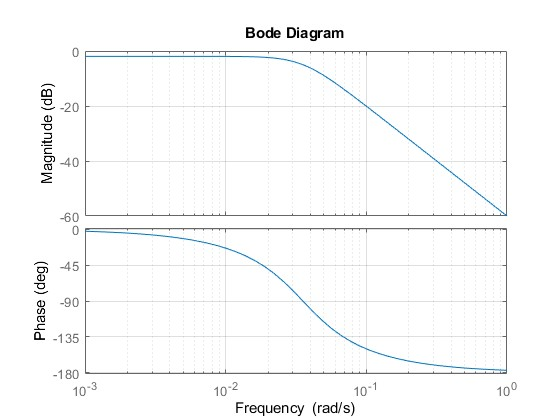
\includegraphics[width=0.75\textwidth]{immagini/bode.jpg}
    \caption{Diagramma di bode di G}
    \label{fig:transform_bode}
\end{figure}

\section{Mappatura specifiche del regolatore}
\label{sec:specifications}

Le specifiche da soddisfare sono
\begin{itemize}
	\item[1)] Errore a regime $\lvert e_\infty \rvert \le e^* = 0.01$ in 
        risposta a un gradino $w(t) = 2 \cdot 1(t)$ e $d(t) = 2 \cdot 1(t)$.\\
 
	\item[2)] Per garantire una certa robustezza del sistema si deve 
        avere un margine di fase $M_f \ge 30^{\circ}$.\\

        \item[3)] Il sistema può accettare una sovraelongazione percentuale al massimo dell'$1 \%$ : $S \% \le 1 \%$.\\

        \item[4)] Il tempo di assestamento all' $\epsilon \% = 1 \%$ deve essere inferiore al valore fissato: $T_{a,\epsilon} = 1s$.\\

        \item[5)] Il disturbo in uscita $d(t)$ con una banda limitata nel range di pulsazioni [0,0.1], deve essere \\abbattuto di almeno $35_{dB}$.\\
        
	\item[6)] Il rumore di misura $n(t)$, con una banda limitata nel 
        range di pulsazioni $[10^3,10^6]$, deve essere abbattuto di almeno $80_{dB}$.\\
\end{itemize}
%
Andiamo ad effettuare la mappatura punto per punto delle specifiche richieste.

\begin{itemize}
    %Prima specifica
    \item[1)] Al punto uno ci viene richiesto un $e_\infty \le 0.01$ tenendo come riferimento un gradino in ingresso $w(t) = 2 \cdot 1(t)$ e un disturbo in uscita pari a un gradino $d(t) = 2 \cdot 1(t)$.\\\\
    L'errore a regime è definito come
    \begin{equation}\label{eq:errore a regime}
        e_\infty = \lim_{t \to \infty} e(t)
    \end{equation}
    con $e(t) = w(t) - y(t)$ ricavato dal fatto che consideriamo un sistema in retroazione.\\\\
    Attraverso l'utilizzo del Teorema del Valore Finale possiamo riscrivere \eqref{eq:errore a regime} come
    \begin{equation}\label{eq:errore a regime laplace}
        e_\infty = \lim_{s \to 0} s \cdot E(s)
    \end{equation}
    Utilizzando le funzioni di sensitività ricavate dallo studio del sistema in retroazione e tenendo per adesso solo in considerazione l'ingresso di riferimento possiamo scrivere $E(s)$ come:
    \begin{equation*}
        E(s) = E_w(s) = S(s) \cdot W(s) 
    \end{equation*}
    quindi è possibile riscrivere \eqref{eq:errore a regime laplace} come:
    \begin{align*}
        e_{\infty,w} = \lim_{s \to 0} s \cdot S(s) \cdot W(s) 
        \\
        e_{\infty,w} = \lim_{s \to 0} s \cdot S(s) \cdot \frac{W}{s}
        \\
        e_{\infty,w} = W \cdot \lim_{s \to 0} S(s)
    \end{align*}
    Focalizzandoci adesso sul $\lim_{s \to 0} S(s)$ può essere riscritto attraverso l'utilizzo della forma fattorizzata di $L(s)$ ovvero $L(s) = \frac{N_L(s)}{D_L(s)}$ e si ricava che:
    \begin{equation*}
        \lim_{s \to 0} \frac{s^g}{\mu + s^g}
    \end{equation*}
    Considerando il fatto che non è conveniente avere poli nell'origine poichè abbasserebbero ancora di più la fase pongo $g = 0$ e ne ricavo che:
    \begin{equation*}
        e_{\infty,w}= W \cdot \lim_{s \to 0} \frac{1}{\mu + 1} = \frac{W}{1 + \mu}
    \end{equation*}
    Effettuando adesso lo stesso ragionamento per il disturbo in uscita $d(t)$ ricaviamo che:
    \begin{equation*}
        e_{\infty,d} = \frac{D}{1 + \mu}
    \end{equation*}
    e che quindi possiamo scrivere l'errore a regime come
    \begin{subequations}
    \begin{align}
        &e_\infty = \frac{W + D}{1 + \mu} \approx \frac{W +D}{\mu} \le e^* = 0.01
        \\
        &\mu \ge \frac{W + D}{0.01} = \frac{2 + 2}{0.01} = 400 
        \label{eq:guadagno_minimo}
    \end{align}
    \end{subequations}
    Abbiamo ricavato il guadagno minimo di $L(s)$ per poter avere un errore a regime uguale a $0.01$
    \begin{equation*}
        L(0) = \mu = 400
    \end{equation*}

    %Seconda specifica
    \item[2)] In questo punto delle specifiche ci viene richiesto di far si che la nostra $L(s)$ abbia un margine di fase $M_f \ge 30^{\circ}$ e quindi ne terremo conto durante la progettazione del regolatore

    %Terza Specifica
    \item[3)] In questo punto ci viene richiesto che il nostro sistema abbia al massimo una $S \% \le S^* = 1 \% = 0.01$.
    \\
    \\
    Se progettiamo $L(s)$ in modo che $F(s)$ abbia una coppia di poli c.c. dominanti in $\omega_n \approx \omega_c$ con coefficiente di smorzamento $\xi$ allora possiamo approssimare ques'ultimo come
    \begin{equation*}
        \xi \approx \frac{M_f}{100}
    \end{equation*}
    Essendo il nostro un sistema del $2^{\circ}$ ordine con una coppia di poli complessi coniugati rispettivamente in 
    \begin{equation*}
        p_1 = -0.025 + 0.025i \ \ \ \ \
        p_2 = -0.025 - 0.025i
    \end{equation*}
    posso scrivere $S^*$ come 
    \begin{equation*}
        S^* = e^{\frac{- \pi \xi^*}{\sqrt{1 - (\xi^*)^2}}} = 0.01.
    \end{equation*}
    Per far si che $S \% \le S^*$ occorre far si che $\xi \ge \xi^*$, quindi adesso ricaveremo $\xi^*$ attraverso l'utilizzo di $S^*$
    \begin{equation*}
        \xi^* = \sqrt{\frac{(\ln(S^*))^2}{\pi^2 + (\ln(S^*))^2}} = 
        \sqrt{\frac{(\ln(0.01))^2}{\pi^2 + (\ln(0.01))^2}} = 0.8261
    \end{equation*}
    Trovato $\xi^*$ e sapendo che $\xi \ge \xi^*$ possiamo arrivare alla seguente conclusione 
    \begin{equation*}
        \xi^* \le \xi \approx \frac{M_f}{100} \implies M_f \ge 100 \cdot \xi^* = 82.61
    \end{equation*}
    Siamo arrivati alla conlusione che per far si che $L(s)$ abbia una $S \% \le 0.01$ occorre che
    \begin{equation*}
        M_f \ge 82.61
    \end{equation*}
    Abbiamo trovato che il margine di fase per la sovraelongazione percencentuale è maggiore del margine di fase richiesto da progetto, quindi l'abbiamo automaticamente rispettato.

    %Quarto punto 
    \item[4)] In questo punto ci viene richiesto che il tempo di assetamento a $\epsilon = 1 \%$, ovvero $T_{a,1}$, sia inferiore a $1s$.
    \\
    \\
    Considerando il fatto che il nostro sistema è del $2^{\circ}$ ordine possiamo approssimare $T_{a,1}$ come
    \begin{equation*}
        T_{a,1} \approx \frac{4,6}{\xi \omega_n}
    \end{equation*}
    e da qui ricaviamo che 
    \begin{equation*}
        \xi \omega_n \ge \frac{4.6}{T^*} = \frac{4,6}{1} = 4.6
    \end{equation*}
    Ora sapendo che $\xi \approx \frac{M_f}{100}$ posso arrivare alla conclusione che 
    \begin{equation*}
        \omega_n \ge \frac{460}{M_f} = \frac{460}{82.61} = 5.5684
    \end{equation*}
    Ricordandoci che nel punto precedente abbiamo supposto $\omega_n \approx \omega_c$ possiamo scrivere che
    \begin{equation*}
        \omega_c \ge 5.5684
    \end{equation*}
    con $\omega_c$ intesa come pulsazione di attraversamento in 0 dB.
    \\
    \\
    In conclusione abbiamo trovato la pulsazione minima sotto il quale non possiamo attraversare gli 0 dB per poter progettare il nostro regolatore.

    %Quinto punto
    \item[5)] In questo punto ci viene richiesto di attenuare il disturbo in uscita $d(t)$ di $35_{dB}$ nel range di pulsazioni tra $[0, 0.1]$.
    \\
    \\
    Attraverso l'utilizzo delle funzioni di sensitività, in particolare di $S(j\omega)$ che ci consente di lavorare direttamente sul disturbo in uscita, possiamo dire che per far si che $d(t)$ sia attenuato di $35_{dB}$ dobbiamo osservare lo studio in frequenza di $S(j\omega)$, ovvero
    \begin{equation*}
        |S(j\omega)|_{dB} =
        \begin{cases}
            -|L(j\omega)|_{dB} & \text{se $\omega \le \omega_c$} \\
            1_{dB} & \text{se $\omega > \omega_c$}
        \end{cases}
    \end{equation*}
    e sapendo che $\omega_{d,max} \ll \omega_c$ possiamo concludere che per far si che $S(j\omega)$ vada ad attenuare $d(t)$ occorre che
    \begin{equation*}
        |L(j\omega)|_{dB} \ge 35_{dB}
    \end{equation*}
    nel range di pulsazioni dato dalle specifiche.

    %Sesto punto
    \item[6)] In questo punto ci viene richiesto di attenuare di almeno $80_{dB}$ il disturbo di misura $n(t)$ che ha un range di pulsazioni tra $[10^3,10^6]$.
    \\
    \\
    Attraverso l'utilizzo delle funzioni di sensitività, in particolare di $F(j\omega)$ che ci consente di lavorare direttamente sul disturbo di misura, possiamo dire che per far si che $n(t)$ sia attenuato di $80_{dB}$ dobbiamo osservare lo studio in frequenza di $F(s)$, ovvero
    \begin{equation*}
        |F(j\omega)|_{dB} =
        \begin{cases}
            1_{dB} & \text{se $\omega \le \omega_c$} \\
            |L(j\omega)|_{dB} & \text{se $\omega > \omega_c$}
        \end{cases}
    \end{equation*}
    e sapendo che $\omega_c \ll \omega_{n, min}$ possiamo concludere che per far si che $F(j\omega)$ vada ad attenuare $n(t)$ occorre che
    \begin{equation*}
        |L(j\omega)|_{dB} \le -80_{dB}
    \end{equation*}
    nel range di pulsazioni dato dalle specifiche.
\end{itemize}
Pertanto, dopo aver effettuato le varie osservazioni sulle specifiche, mostriamo il diagramma di Bode della funzione di trasferimento $G(s)$ con le zone proibite emerse dalla mappatura delle specifiche.

\begin{figure}[H]
    \centering
    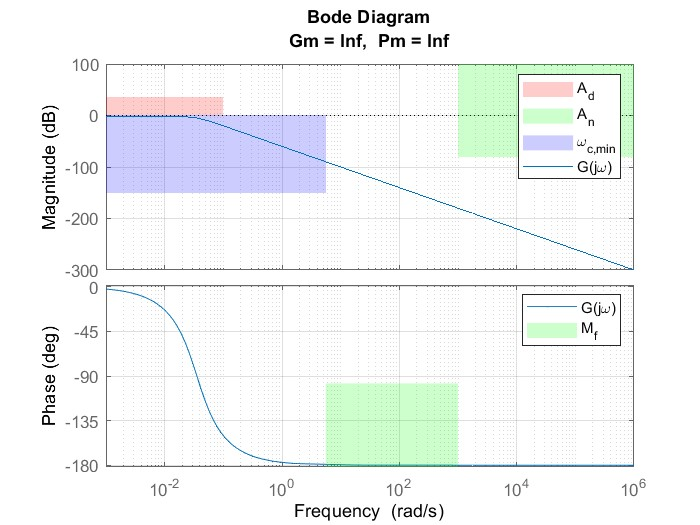
\includegraphics[width=0.70\textwidth]{immagini/specifiche.jpg}
    \caption{Diagramma di bode di G(s) con specifiche}
    \label{fig:specifiche}
\end{figure}


\section{Sintesi del regolatore statico}
\label{sec:static_regulator}
%
    In questa sezione progettiamo il regolatore statico $R_s(s)$ partendo dalle analisi fatte in sezione~\ref{sec:specifications}.
    \\\\
%
    Dalle analisi sull'errore a regime (vedi \ref{eq:guadagno_minimo}) emerge che il valore minimo prescritto per L(0) 
    \begin{subequations}
    \begin{align*}
        &\mu = 400
    \end{align*}
    \end{subequations}
    
    La risposta in frequenza della funzione di trasferimento del sistema linearizzato calcolata in zero è pari a
    \begin{subequations}
    \begin{align*}
        &G_0 = 0.80
    \end{align*}
    \end{subequations}

    Quindi il guadagno minimo del regolatore viene ottenuto come L(0)/G(0)
    \begin{align*}
         &R_s(s) = \mu / G_0 = 500
    \end{align*}
%
    Dunque, definiamo la funzione estesa $Ge = R_s(s) \cdot G(s)$ e, in Figura \ref{fig:static_regulator}, mostriamo il suo diagramma di Bode per verificare se e quali zone proibite vengono attraversate.
    
\begin{figure}[H]
    \centering
    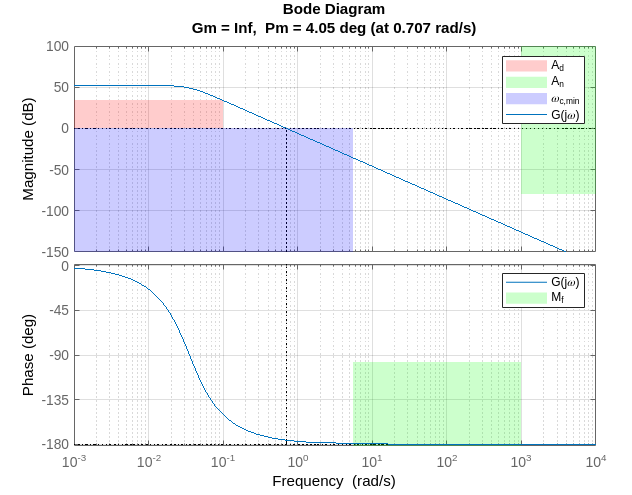
\includegraphics[width=0.75\textwidth]{immagini/regolatore_statico.png}
    \caption{Diagramma di G estesa}
    \label{fig:static_regulator}
\end{figure}
%
    Da Figura \ref{fig:static_regulator}, emerge che nell'intervallo 
    in cui possiamo attraversare gli 0 dB la fase si trova sempre sotto al margine di fase imposto come limite.


\section{Sintesi del regolatore dinamico}

In questa sezione, progettiamo il regolatore dinamico $R_d(s)$. 
%
    Dalle analisi fatte in Sezione~\ref{sec:static_regulator}, notiamo di essere nello Scenario di tipo B.
    \\\\
    Per questo motivo, inizialmente, abbiamo deciso di realizzare il nostro regolatore dinamico come una rete anticipatrice
    \begin{equation*}
        R_d(s)=\dfrac{1+\tau s}{1+\alpha \tau s}
    \end{equation*}
    Per progettare la rete anticipatrice abbiamo imposto la pulsazione di attraversamento degli 0dB all'interno del range definito da $\omega_{c_{min}}, \omega_{c_{max}}$. In particolare abbiamo preso 
    $\omega_c^*=\omega_{c,min}+1 \textrm{ rad/s}$  e $M_f^*=M_f+5$ gradi.
    $\\\\$
    In seguito abbiamo calcolato $M^*,\varphi^*,\tau \textrm{ e } \alpha \tau$ usando le formule di inversione:
    \begin{align*}
        &\omega_c^*=6.5684  \textrm{ rad/s}\\
        &M_f=\ang{87.6085} \textrm{ gradi}\\
        &M^* = 10^{-\dfrac{\lvert G_e(j \omega_c^*) \lvert_{dB}}{20}} \simeq 86.2886\\
        &\varphi^*= \ang{87.1724}\\
        &\alpha \tau = \dfrac{\cos \varphi^* - \frac{1}{M^*}}{\omega_c^* \sin \varphi^*}=0.0058\\
        &\tau = \dfrac{M^*-\cos \varphi^*}{\omega_c^* \sin \varphi^*}=13.1454
    \end{align*}
    $\\$
    In questa prima fase, i valori calcolati di $\alpha \tau$ e $\tau$ ci permettono di definire il regolatore dinamico.\\
    Per verificare che i vincoli siano rispettati dobbiamo osservare il comportamento della funzione
    $L(s)$:
    \begin{equation*}
        L(s)=R(s)G(s)=R_d(s)R_s(s)G(s)
    \end{equation*} 
    Verifichiamo il comportamento di L(s) tramite il suo diagramma di Bode. \\Osserviamo dalla figura  \ref{fig:regd1} che attraverso la rete anticipatrice siamo riusciti ad attraversare gli 0dB all'interno del range definito da $\omega_{c_{min}}, \omega_{c_{max}}$ e a rispettare il margine di fase, ma non  viene rispettata la specifica  sull'abbattimento del rumore di misura n(t). 
     \begin{figure}[H]
    \centering
    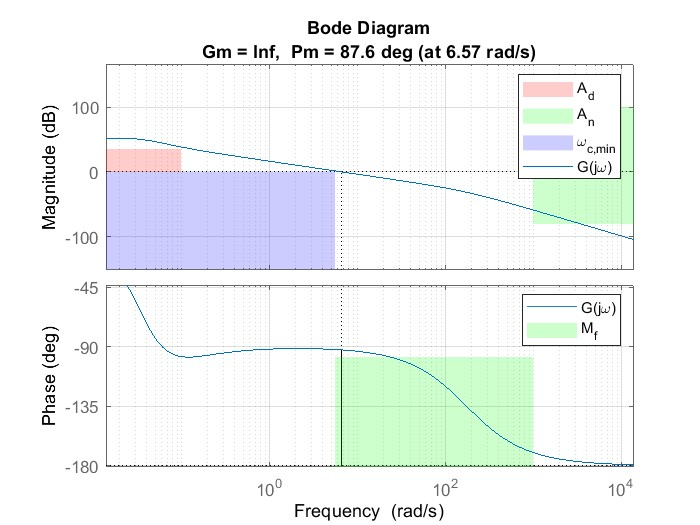
\includegraphics[width=0.70\textwidth]{immagini/regolatore1.jpg}
    \caption{Diagramma di Bode di L(s) con rete anticipatrice}
    \label{fig:regd1}
\end{figure}
    
    Per questo motivo abbiamo deciso di aggiungere un polo reale negativo in modo da abbasare l'ampiezza in alte frequenze e mantenere la fase il più costante possibile. 
    \\
    \begin{equation*}
        Polo(s)=\dfrac{1}{1+ \sigma s}
    \end{equation*}
Nello specifico abbiamo imposto $\sigma=1/80
    $.\\
    In questo modo il nostro regolatore dinamico diventa:
    \begin{equation*}
        R_d(s)=\dfrac{1+\tau s}{1+\alpha \tau s} \cdot\dfrac{1}{1+ \sigma s}
    \end{equation*}
Verifichiamo nuovamente il comportamento di L(s) tramite il suo diagramma di Bode. \\Osserviamo dalla figura  \ref{fig:regdgiusto} che attraverso la rete anticipatrice e il polo reale negativo la funzione in anello aperto rispetta i vincoli imposti.
    
     \begin{figure}[H]
    \centering
    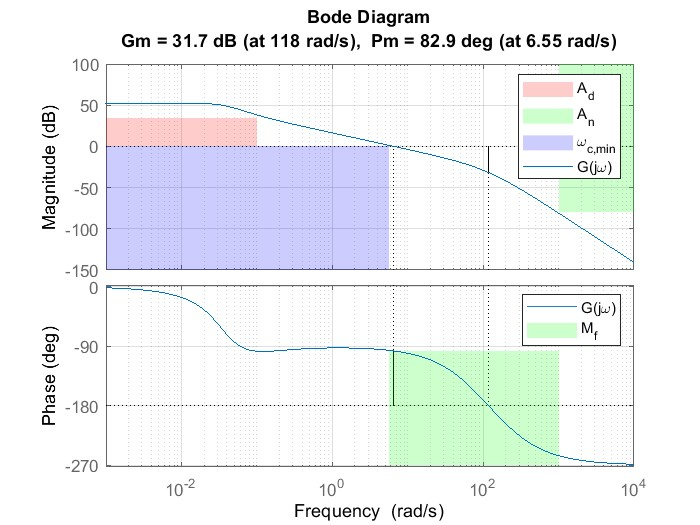
\includegraphics[width=0.75\textwidth]{immagini/regolatore2.jpg}
    \caption{Diagramma di Bode di L(s) con rete anticipatrice e polo}
    \label{fig:regdgiusto}
\end{figure}

Infine abbiamo verificato che il sistema in anello chiuso rispetti le specifiche.\\
La funzione in anello chiuso $F(s)$ è rappresentata dal seguente Diagramma di Bode

\begin{figure}[H]
    \centering
    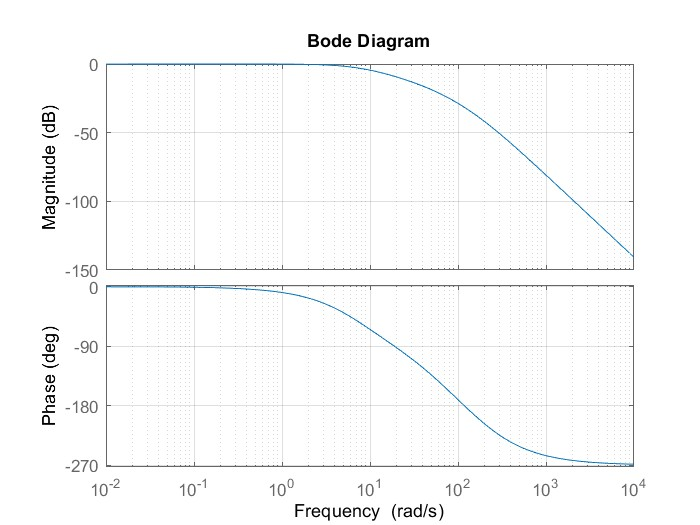
\includegraphics[width=0.70\textwidth]{immagini/F_s.jpg}
    \caption{Diagramma di Bode di F(s)}
    \label{fig:F_s}
\end{figure}

Nella seguente figura \ref{fig:test_gradino} si può osservare che abbiamo testato il sistema in anello chiuso con l'ingresso a gradino citato nelle specifiche della sezione \ref{sec:specifications} e riportando i vincoli di sovraelongazione e tempo di assestamento.

\begin{figure}[H]
    \centering
    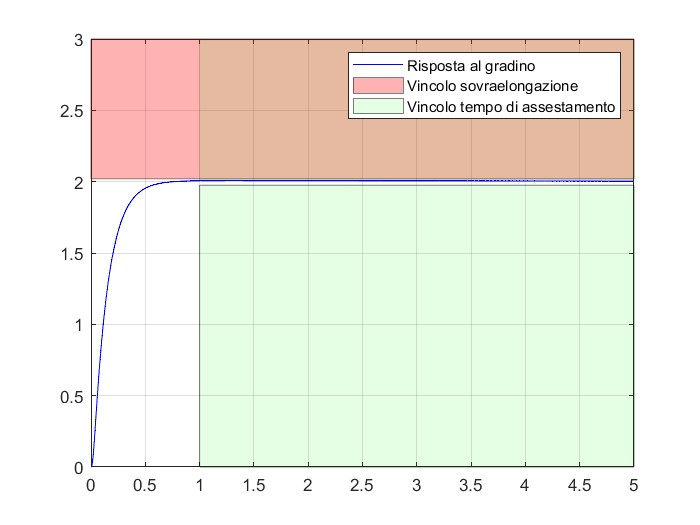
\includegraphics[width=0.70\textwidth]{immagini/risposta_al_gradino_test_punto_3.jpg}
    \caption{Test gradino}
    \label{fig:test_gradino}
\end{figure}
   
\section{Test sul sistema linearizzato}
In questa sezione, testiamo il sistema di controllo sul sistema linearizzato con i seguenti ingressi:
    \begin{subequations}
    \begin{equation}
    \label{eq:ingressogradino}
         w(t)=-2 \cdot 1(t)\\
    \end{equation}
    \begin{equation}\label{eq:ingressod}
         d(t)=\sum_{k=1}^{4} 0.3\cdot \sin(0.025kt)\\
    \end{equation}
    \begin{equation}\label{eq:ingresson}
        n(t)=\sum_{k=1}^{4} 0.2 \cdot  \sin(10^{3} kt)\\
    \end{equation}
    \end{subequations}
Sfruttando il principio di sovrapposizione degli effetti:
\begin{center}
Y(s) = $Y_\omega(s) + Y_d (s) + Y_n (s)$
\end{center}
Possiamo studiare la risposta del sistema ai precedenti ingressi come somma delle singole risposte ai singoli ingressi. In particolare:
\begin{itemize}
\item $Y_\omega(s)$ uscita con ingresso $w(t)$\eqref{eq:ingressogradino} e ponendo D(s) e N(s) = 0\\
Utilizziamo la funzione di sensitività complementare portando in ingresso $w(t)$\eqref{eq:ingressogradino}\\
\begin{center}
F(s) =$  \frac{R(s) \cdot G(s)}{1+ R(s) \cdot G(s)} $
\end{center}

 \begin{figure}[H]
    \centering
    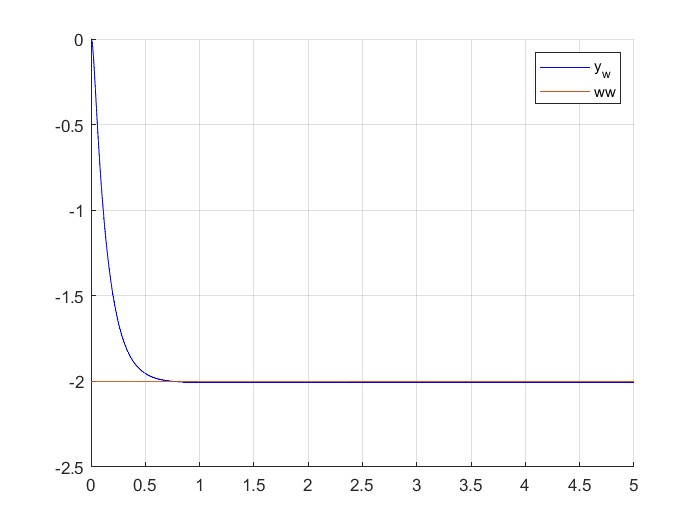
\includegraphics[width=0.75\textwidth]{immagini/risposta_al_gradino_punto_4.jpg}
    \caption{Risposta al gradino}
\end{figure}
 \item $Y_d (s)$ uscita con ingresso $d(t)$\eqref{eq:ingressod} e ponendo W(s) e N(s) = 0\\
Nel secondo caso utilizziamo la funzione di sensitività portando in ingresso $d(t)$\eqref{eq:ingressod}\\
\begin{center}
S(s) =$  \frac{1}{1+ R(s) \cdot G(s)} $
\end{center}
\begin{figure}[H]
    \centering
    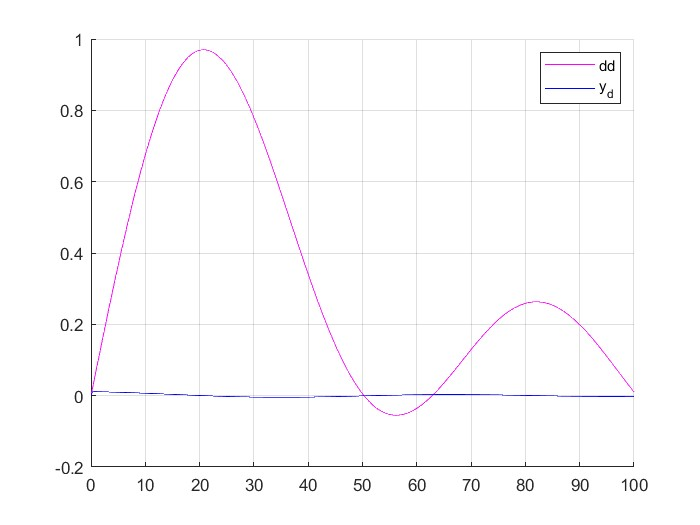
\includegraphics[width=0.75\textwidth]{immagini/disturbouscita.jpg}
    \caption{Risposta al disturbo in uscita}
\end{figure}
\item $Y_n (s)$ uscita con ingresso $n(t)$\eqref{eq:ingresson} e ponendo W(s) e D(s) = 0\\
Nel terzo caso utilizziamo la funzione di sensitività complementare negata, in ingresso $n(t)$\eqref{eq:ingresson}
\begin{center}
F(s) =$ \frac{R(s) \cdot G(s)}{1+ R(s) \cdot G(s)} $
\end{center}
 \begin{figure}[H]
    \centering
    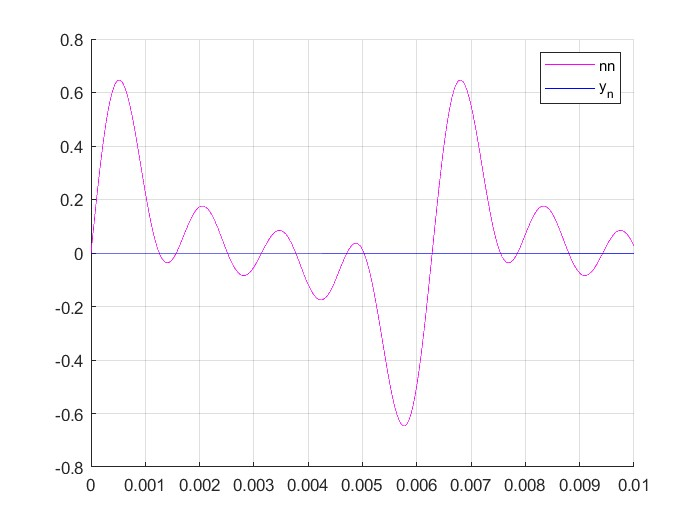
\includegraphics[width=0.75\textwidth]{immagini/disturborumore.jpg}
    \caption{Risposta al disturbo di rumore}
\end{figure}
\end{itemize}

Attraverso l'utilizzo di simulink siamo andati a realizzare uno schema a blocchi contenente il sistema linearizzato e a testarlo con tutti gli ingressi in contemporanea.
\\
\begin{figure}[H]
    \centering
    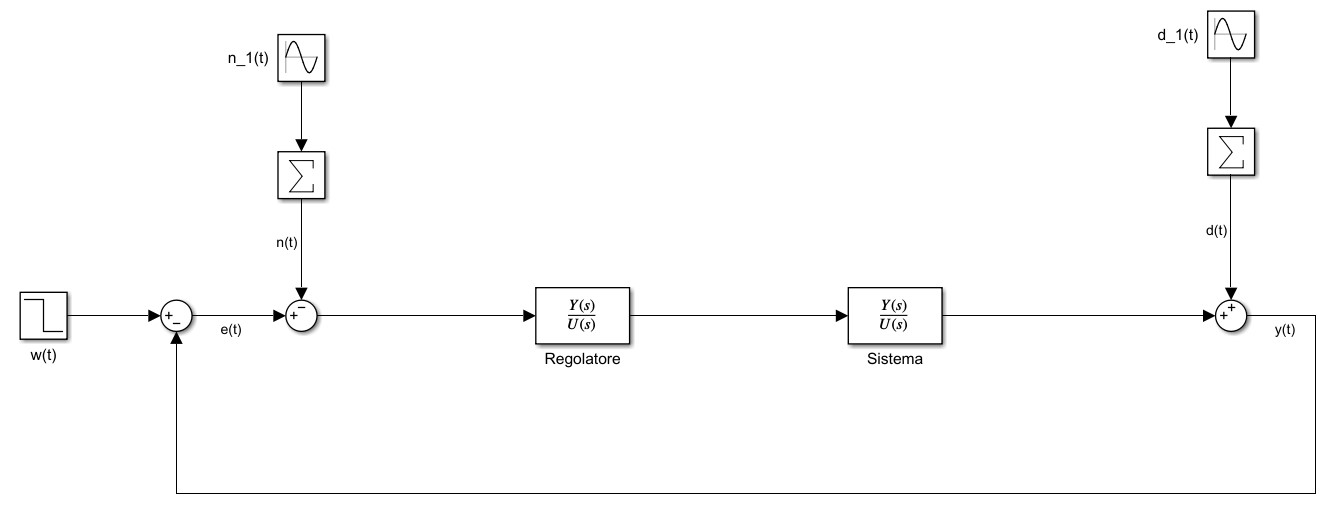
\includegraphics[width=0.75\textwidth]{immagini/simulink_sistema_linearizzato.jpg}
    \caption{Schema a blocchi del sistema linearizzato}
    \label{sys_linearizzato}
\end{figure}

\begin{figure}[H]
    \centering
    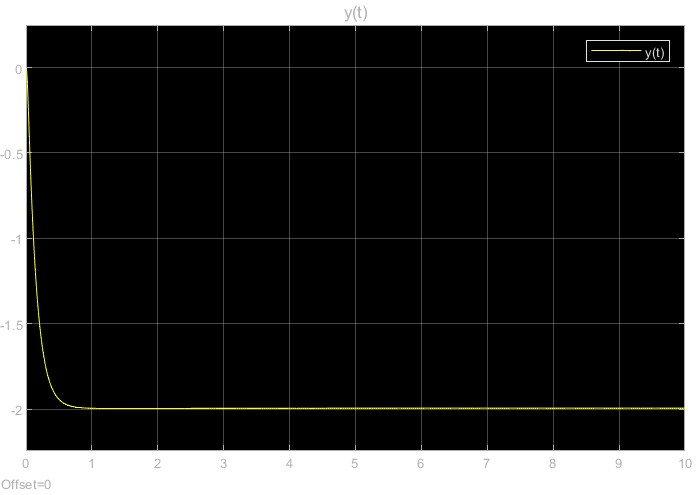
\includegraphics[width=0.75\textwidth]{immagini/risposta_sistema_a_tutti_gli_ingressi.jpg}
    \caption{Risposta del sistema linearizzato}
    \label{risposta_sys_linearizzato}
\end{figure}






\section{Test sul sistema non lineare}
In questa sezione, testiamo l'efficacia del controllore progettato sul modello non lineare.
\\
\\
Tramite l'utilizzo di Simulink abbiamo sviluppato il seguente schema a blocchi
\begin{figure}[H]
    \centering
    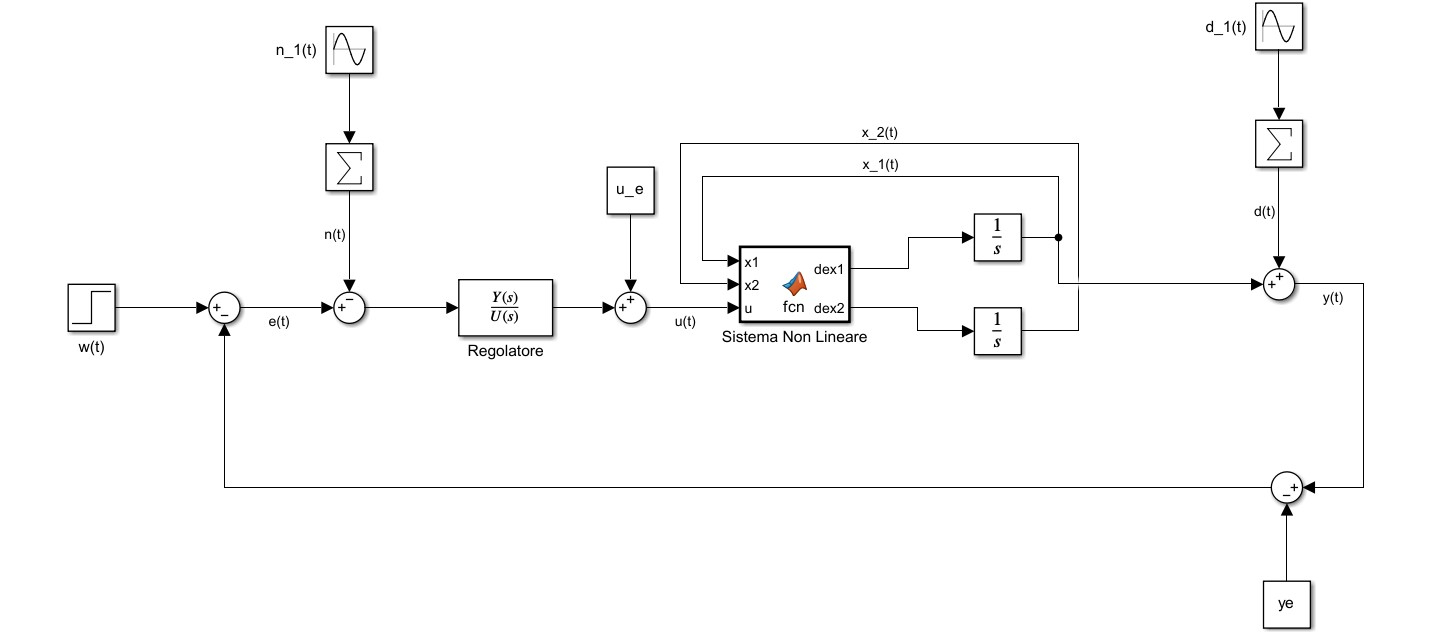
\includegraphics[width=0.75\textwidth]{immagini/test_sistema_non_linearizzato.jpg}
    \caption{Schema a blocchi per test su sistema non lineare}
    \label{fig:simulink_sistema_non_linearizzato}
\end{figure}
Nel blocco "Sistema Non Lienare" abbiamo inserito il nostro sistema non linearizzato tramite l'utilizzo del seguente codice:\\
\\
\texttt{function [dex1,dex2] = fcn(x1,x2,u)}\\
\texttt{\%Parametri}\\
\texttt{beta = 0.5;}\\
\texttt{J = 10;}\\
\texttt{a = 0.01;}\\
\texttt{F\_v = -5;}\\
\\
\texttt{\%Sistema}\\
\texttt{dex1 = x2;}\\
\texttt{dex2 = (-beta/J)*x2+(a/(2*J))*sin(x1)*F\_v+(a/J)*u;}\\
\\
Abbiamo usato come riferimento $w(t)$, rumore di uscita $d(t)$ e di misura $n(t)$ quelli specificati nel punto precedente.\\
Oltre a ciò abbiamo impostato come stato iniziale del sistema lo 
stato di equilibrio (specificato mediante i blocchi integratori), ottenendo come risposta:
\begin{figure}[H]
    \centering
    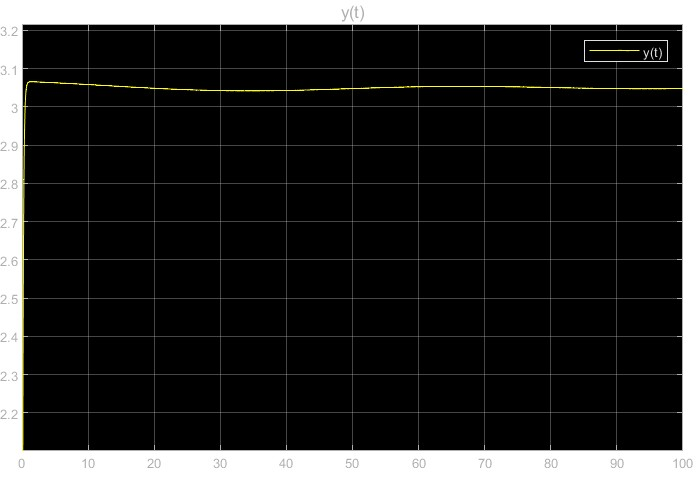
\includegraphics[width=0.60\textwidth]{immagini/risposta_sistema_non_linearizzato.jpg}
    \caption{Risposta del Sistema non Linearizzato}
\label{fig:risposta_sistema_non:linearizzato}
\end{figure}

\section{Conclusioni}
In conclusione abbiamo verificato la realizzabilità del sistema di controllo che manovra il drone nel rispetto delle specifiche imposteci dal progetto.\\ Abbiamo superato tutti i test, ciò è stato possibile attraverso il regolatore statico e dinamico, in particolare con il regolatore statico siamo andati a rispettare le specifiche a regime, mentre con quello dinamico tutte le specifiche in transitorio.
\end{document}